\documentclass[12pt, a4paper]{report}
\usepackage[utf8]{inputenc}
\usepackage{graphicx}
\usepackage{natbib}

\title{Virtual Arduino}
\author{Ahmed Sabbah}
\date{14 April 2011}

\begin{document}

\maketitle
\begin{abstract}
Virtual Arduino is a desktop application that simulates the Arduino board. It is mainly an educational tool that aims to provide hands-on experience for embedded systems programming and hardware beginners. This application provides an experience as close as possible to the real life. Through this application, the user can write Arduino code, compile and apload it to a virtual Arduino. He can also implement circuits, add hardware components and connect them to the Arduino. It also provides visualization for the output the Arduino reflects on the circuits and hardware components.
\end{abstract}


\chapter{Introduction}
A microcontroller is an integrated chip that is often part of an embedded system. Microcontroller evaluation boards are considered an efficient way to learn embedded systems programming as it provides hands-on experience to the user. The use of these boards provides the opportunity to learn to program and implement hardware circuits. The challenge nowadays is to decrease the cost of hardware components building these boards. The cost problem is very effective mainly in the educational purposes, where many students don’t have access to the boards. Our proposal is to make a real time hardware simulator as close as possible to the real experience. It provides a simulation for this hands-on experience the boards give. The simulator covers all aspects of an embedded system including hardware components, hardware interfacing, hardware failure, board setting, code compilation and uploading. The proposal is to implement this simulator for the Arduino Uno evaluation board. The Arduino Uno is a board based on the ATmega328 microcontroller. Several simulators for Arduino have been implemented, but none of them can replace the real life experience of the actual board and hardware components. The main aim of this simulator is to provide an experience as close as possible to the real life. The user will be able to write and compile Arduino code to a virtual Arduino. He will also be able to implement the circuitry and hardware components virtually and connect them to the virtual Arduino. A scalable library with the most common hardware components is provided. He can as well see the output of his implementation virtually as supposed to be in real life. Thus providing him with experience as close as possible to real life without needing to buy the board or any other components.


\chapter{Background}
In this section, the architecture of the project is discussed. The requirements of the application and elements are included in details. To simulate the experience virtually, The application will have three main modules, represented in (Figure 2.1).

\begin{figure}[h!]
\centering
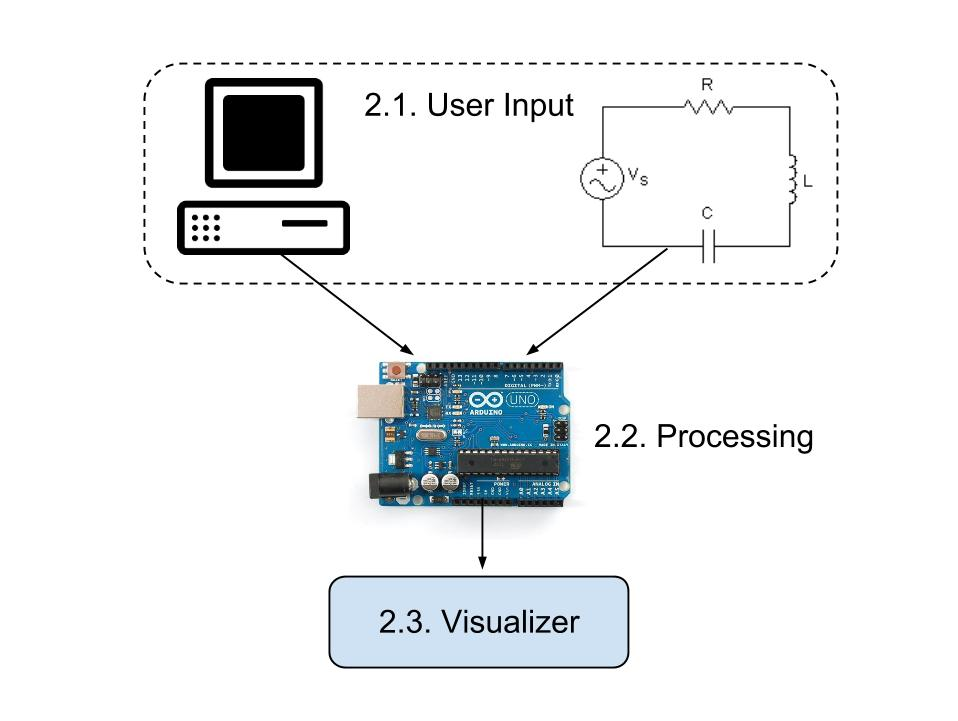
\includegraphics[height=9cm, width=12cm]{Architecture.jpg}
\caption{Virtual Arduino Architecture}
\label{Architecture}
\end{figure}

\section{User Input Modules}
This module is the first level of the program’s architecture. It represents all forms of input the user can give. This input can be in the form of Arduino code or circuitry.
\subsection{Computer Module}
This module represents the computer related Arduino user experience, where the user writes Arduino code through the Arduino IDE as in real life. The code is compiled through the IDE as well. Instead of uploading the code to a real Arduino, the user uploads it to the virtual Arduino. Uploading the code into the Arduino in real life is done by sending a hex code file to the serial port connected to the Arduino through USB connection. This will done virtually in the simulator by creating a virtual serial port and sending the code to it through the Arduino IDE and receiving it in The simulator application by reading from this port.
\newpage
\subsection{Circuitry Module}
This module represents the hardware part of working with Arduino. The user can build circuits and add hardware components to it. He can also connect these circuits to the Arduino through the Arduino ports. To implement this module, three main components will be implemented.
\subsubsection{Components Library}
A scalable hardware library will be implemented from where the user can use components to build circuits. The library will be divided into four categories Input, Idle, Power and Output components. Also the user will be able to vary the input sensing components which will reflect on the Arduino behavior.
\subsubsection{Circuit Builder}
This part is all about simulating the real life experience of implementing circuits and adding hardware components to it. The user will have a workspace where he can implement circuits as close as possible to how he does in real life. He can make circuits and connect hardware components using the library available.
\subsubsection{Circuit Simplifier}
In this section, the circuit is toned down leaving only the effective components on which the output appears.
\section{Processing Module}
This is the second level of the architecture which processes the inputs it gets from the first module. It takes instructions from the IDE through the virtual serial port and the simplified circuit and evaluates the state of the output components. It then sends these states to the visualizer module. This module is discussed later with more details in (Chapter 3.0).
\newpage
\section{Output Visualizer}
In this module the user will be able to visualize the output of the code on the hardware components. This module uses the results from the previous module and reflects them on the Arduino board, circuitry and hardware components.
\subsection{Success Scenario Visualizer}
This part simulates the senario when the code compiles and there are no hardware failures. Each component is checked and according to the state it’s output is visualized.
\subsection{Hardware Failure Visualizer}
This senario happens when there are failures caused by the hardware not user. This senario happens a lot in real life. The user will be able to debug the circuits using an avo-meter that will be implemented.
\newpage

\chapter{Processing Module}
This module is mainly a virtual Arduino. It is described by having an Arduino board as a software on the computer. What Arduino board does is receiving a hex code file containing instructions. It executes these instructions and based on these instructions it does changes to its registers, memory components and the circuit connected to it through its ports. Implementing this board is based on implementing the following components.

\section{Arduino Architecture and Components}
The Arduino board to be simulated is the Arduino Uno. Arduino Uno is a microcontroller board based on the ATmega328 datasheet. It has 14 digital input/output pins, 6 analog inputs, 16 MHz crystal oscillator, a USB connection, a power jack, an ICSP header, and a reset button. (Figure 3.1) describes this architecture.

\begin{figure}[h!]
\centering
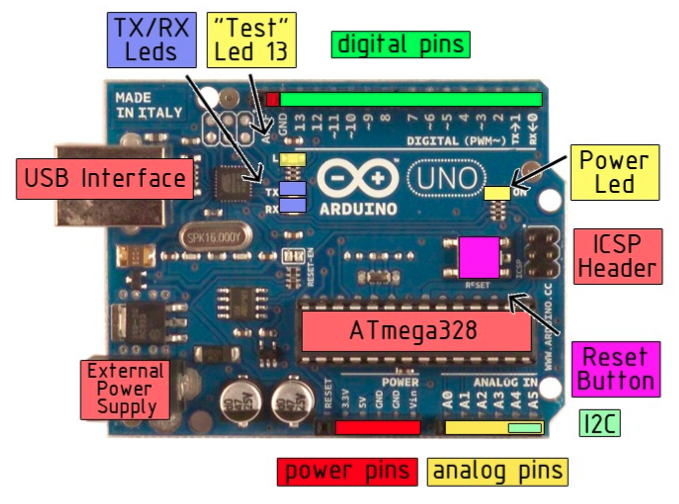
\includegraphics[height=5cm, width=9cm]{UnoBoard.png}
\caption{Arduino Uno Components\protect\cite{ArduinoComponents}}
\label{Arduino Uno}
\end{figure}

\newpage

All These part will be simulated as well as the internal components of Arduino. Arduino Uno contains 32 x 8 General Purpose Working Registers. It also has a Flash Memory of 32 KB, SRAM of 2 KB and an EEPROM of 1 KB. These memory components will also be virtually simulated. (Figure 3.2) is a block diagram for ATmega328.

\begin{figure}[h!]
\centering
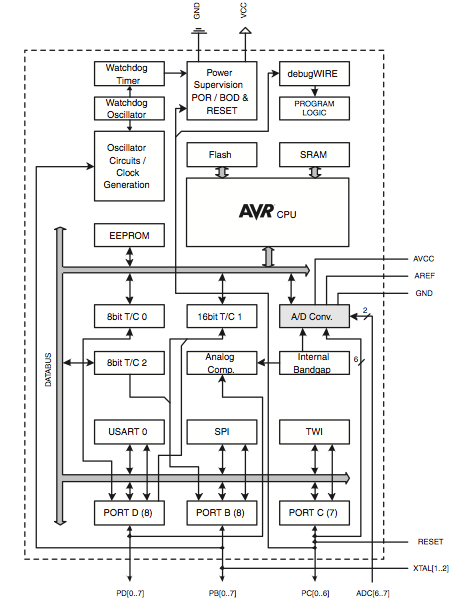
\includegraphics[height=12cm, width=7cm]{ArduinoBlockDiagram.png}
\caption{ATmega block diagram \protect\cite{BlockDiagram}}
\label{Arduino Uno block diagram}
\end{figure}

\newpage

\section{Interpreter for hex code}
Arduino Uno executes hex code of ATmega328 Instruction set. To simulate this part, an interpreter will be implemented which receives these instruction and translate them to actions and data transfer inside the Arduino reflecting on other components. The instruction set for Arduino Uno is available in the ATmega328 datasheet.

\newpage

\chapter{Progress and Strategy}
\section{Progress}
The progress so far is all about defining the project architecture and implementing the Arduino core simulator. All information about Arduino Uno internal hardware and memory components are available. Documentations about the ATmega328 and its instruction set is also available. A sequence diagram describing the interaction between Arduino Internal components is being implemented. Technical decisions were also taken about how to implement the internal memory components of Arduino Uno. A byte in memory components is simulated as an array of eight integers either 0 or 1. So a memory component is an array of arrays of length 8 representing a byte.

\section{Strategy}
Strategy for implementing the Arduino core simulator is implementing an interpreter that translate the hex code Arduino receives into executable commands. Documentation about the instruction set is available for implementing the interpreter. On the other hand, the virtual Arduino architecture will be implemented. Documentations are also available and a sequence diagram is being implemented. By implementing these components, a virtual Arduino board is implemented.


\bibliographystyle{plain}
\bibliography{references.bib}
\end{document}
